\subsection{Mechanism, price and model checks}
The frozen diagnostic suite adds 508 missions. These are exploratory checks;
their intervals are pointwise and are not adjusted across all diagnostic tests.
The mechanism checks pair ten seed blocks across storm and moving-priority
conditions with the shorter radio. Figure~\ref{fig:ablation} reports both
coverage and realized energy.
Energy penalty: mechanism present minus removed changes coverage by -0.477 [-0.692, -0.283] points and energy by -49.5 [-59.2, -39.6] Wh.

Hydraulic fusion family: mechanism present minus removed changes coverage by +1.045 [0.817, 1.309] points and energy by -1.0 [-9.0, 7.2] Wh.

Social recruitment: mechanism present minus removed changes coverage by -0.059 [-0.188, 0.086] points and energy by -1.9 [-5.0, 1.2] Wh.

The no-fusion variant replaces mixed directions with branching-only step
lengths; this changes the proposal family as well as removing the hydraulic
term. It is not a perfectly isolated biochemical-mechanism intervention.
Price checks use the same ten seed blocks at three common energy prices.
These curves expose cost--coverage trade-offs, but do not constitute an
exactly energy-matched or globally optimized Pareto frontier.
\begin{figure*}[tbp]
\centering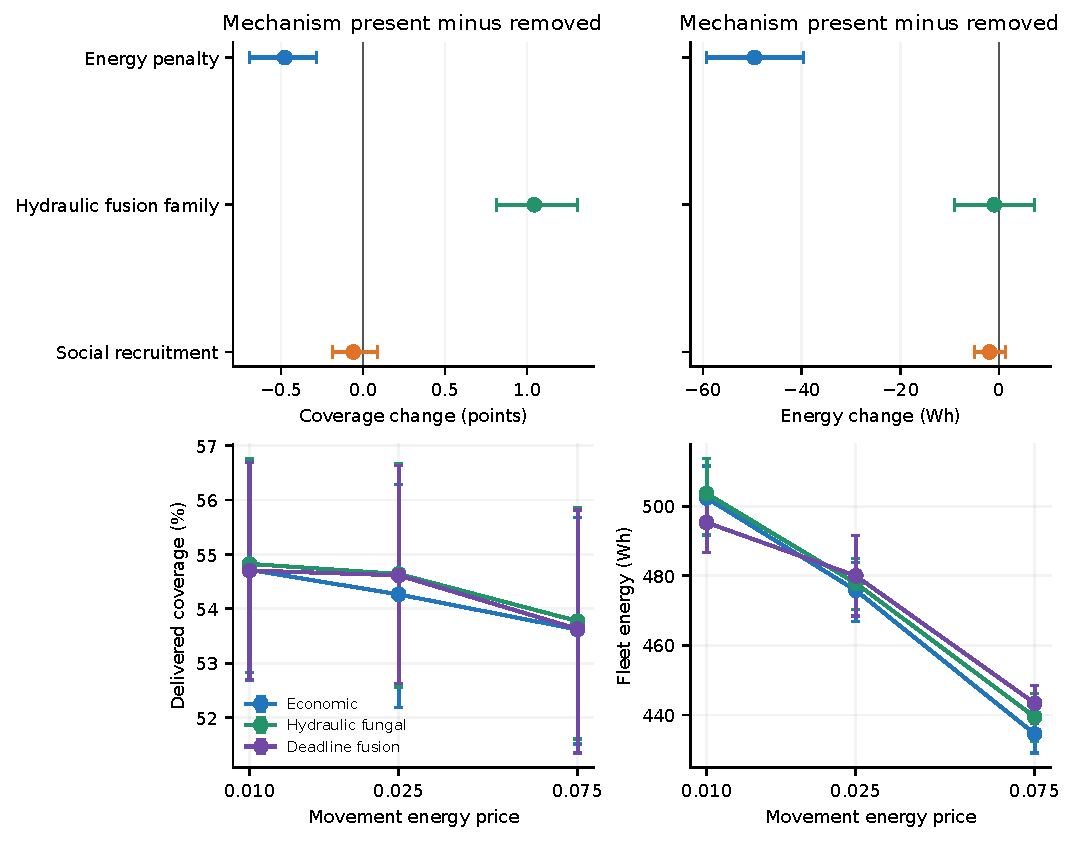
\includegraphics[width=.96\textwidth]{figures/ablation_price.pdf}
\caption{Exploratory mechanism and movement-price checks. Differences use
paired seed blocks; all bars are 95\% bootstrap intervals. Each price point
averages the same ten seeds across two scenarios.}
\label{fig:ablation}
\end{figure*}
\begin{table*}[tbp]
\centering\small\setlength{\tabcolsep}{4pt}
\caption{Diagnostic contrasts with 95\% paired intervals. E: economic; S: tuned
static; H: hydraulic fusion; D: deadline fusion. $n$ counts seed blocks.
Positive energy changes are costs. These are exploratory, pointwise intervals.}
\label{tab:sensitivity}
\begin{tabular}{@{}llrrr@{}}\toprule
Condition & Contrast & $n$ & \shortstack{Coverage change\\(points)} & \shortstack{Energy change\\(Wh)}\\\midrule
\inputtablerows{generated/supplement_table.tex}
\bottomrule\end{tabular}
\end{table*}
Table~\ref{tab:sensitivity} reports altered sensing/correlation, a slower
moving priority, 128-path planning, and calm/blackout controls. The altered-model
case jointly changes the actual detector to a probit curve and increases wave
memory/correlation; it cannot isolate those individual causes. Slower priority
travels at approximately 1.09 m/s, below the 3 m/s vessel limit. The 128-path
check uses only four independent seed blocks and compares policies within that
setting; it is not a paired numerical-convergence test against the 32-path main
study. Negative controls pool the two hardware profiles by seed. A complete
radio blackout prevents delivery irrespective of any formation policy.
The small default biological advantages are not robust across these checks.
Under changed sensing/correlation, both biological coverage intervals include
zero. With slower priority, deadline fusion loses 0.665 coverage points against
hydraulic fusion (interval [-0.934, -0.398]). In the four-seed 128-path check,
hydraulic fusion also underperforms economic control; this small experiment
does not identify numerical integration as the sole cause. Economic control
still improves coverage relative to tuned static in the changed-model and
slower-priority checks, while spending additional energy. These outcomes favor
economic control as the practical baseline and limit claims about biological
performance benefits.

\subsection{Learning pipeline and negative learning result}
A dependency-free linear-softmax REINFORCE policy chooses among nine combinations
of movement step and energy price around the economic controller. Four received
observation frames provide 332 input features for six vessels. The policy sees
cached states, belief summaries and ages, not private true sensor health.
Training uses domain-randomized 40-minute missions. One training seed was run for
50 episodes, evaluated, then resumed for five additional episodes to check
checkpoint continuity. The 50-episode checkpoint is retained separately; the
55-episode checkpoint is not the policy evaluated here.
The 50-episode policy was tested on 18 missions, three scenarios and six paired seed blocks, against constant action 4, which reproduces the neutral economic controller. Coverage changed by -0.805 points (95\% interval [-1.154, -0.397]) and energy by -54.0 Wh ([-80.8, -23.5]). The evaluation utility $\bar C-0.025E/(600\,\mathrm{Wh})$ changed by -0.00581 ([-0.00840, -0.00287]). There is no evidence here that learning improves the mission objective. The energy saving comes with a coverage loss. These small-sample intervals and one training seed do not characterize robust learning performance.
\begin{figure*}[tbp]
\centering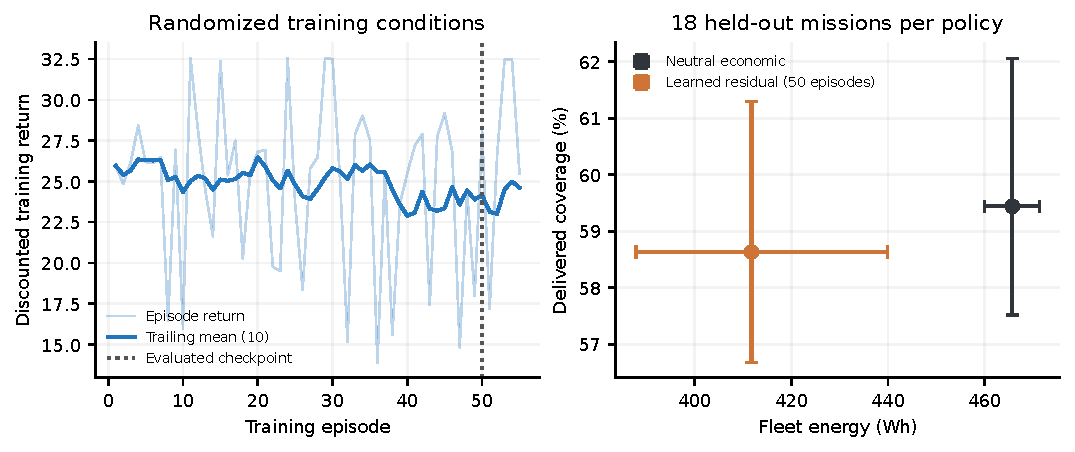
\includegraphics[width=.96\textwidth]{figures/learning.pdf}
\caption{Exploratory learning study. Left: randomized training returns, including
five resume-test episodes after the evaluated checkpoint. A training curve is
not evidence of improved held-out performance. Right: evaluation of the saved
50-episode policy against its neutral economic action; intervals resample six
seed blocks.}
\label{fig:learning}
\end{figure*}
The optional Gymnasium/Stable-Baselines3 PPO environment also passed the
environment checker. PPO was trained for 512 steps, saved, resumed for 128 more,
and loaded for two complete evaluation missions. This 640-step run verifies
the software path only; it is not a substantive PPO efficacy experiment.
The first 512 steps took 129.0 s on the provided CPU environment under concurrent
load (3.97 steps/s). Native training took 505.3 s for the first 50 episodes.
Local hardware should be timed before budgeting longer training.
